%!TEX root = ../report.tex
\section{Echo-SLAM}

\subsection{Sine Sweep Generation}

\subsection{RIR recording}

\subsection{Analysis}

\paragraph{Calibration}

It is required to differentiate the delay induced by the physical distance between microphone, walls and the speakers from the delay induced by the audio system itself. Therefore an analysis of the latency of the audio system is performed. 

For this purpose, the speaker is placed at a well known position with respect to the microphone, so that the physical delay $\Delta t_ph$ can be precisely calculated. It is then sufficient to get the total delay of the signal, $\Delta t_{tot}$ which is composed of the physical delay and the latency ($\Delta t_{tot}=\Delta t_{ph}+\Delta t_{l}$). The total delay is found by sending a reference signal $u_{N1}$ (in this case, a white noise) and recording the response of the microphone, $y_{N2}$.

The response is a scaled and delayed noisy version of the input. Finding the delay comes back to laying the output signal over the input signal with different phase lags until we get a maximum similarity. The lag corresponding to this maximum is the total delay between the input and the output. The tool that performs these steps is the cross-correlation, which, for discrete signals can be written as: 

\begin{equation}
	r_{uy}[k] = \sum\limits_{n=-\infty}^{\infty} u[n]y^*[n-k] \hspace{2em} k=0,\pm1,\pm2,...
\end{equation}

As the cross-correlation is quite computationally expensive, only the first $N_{max}$ samples of both input and output signals are correlated, which is sufficient if we choose $N_{max}$ much bigger than the sample index of the expected delay (for example, $N_{max}=2  \text{ s} \times F_s = 88200$)

\begin{figure}[h!]
	\centering
	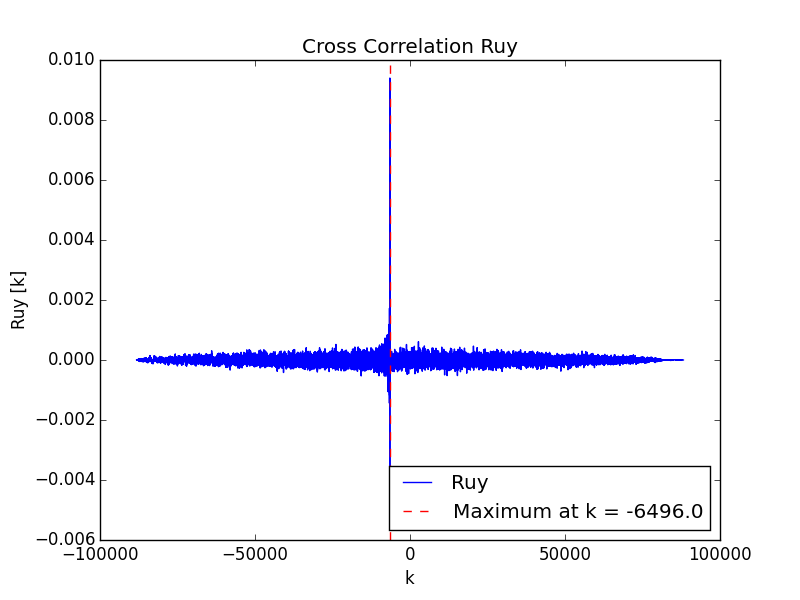
\includegraphics[width=0.8\linewidth]{files/audio_ruy.png}
	\caption{Cross correlation of white noise for latency estimation}
	\label{fig:audio_ruy}
\end{figure}

From Figure \ref{fig:audio_ruy}, we can see that the maximum occurs at sample $k_{max}=-6496$, which corresponds to a delay of $\Delta t_{tot}=k_{max}/F_s=147.3 \text{ ms}$. The distance between microphone and speaker being $d=660mm$, we find $\Delta t_{ph} = d/c=1.9  \text{ ms}$, so the estimated latency of the sound system is about $\Delta t_{l}=145.4 \text{ ms}$.

%\begin{figure}[H]
%	\centering		
%	\begin{subfigure}[b]{0.49\linewidth}
%		\includegraphics[width=\linewidth]{../files/zdot_RefTrackNL.png}
%	\end{subfigure}
%	\begin{subfigure}[b]{0.49\linewidth}
%		\includegraphics[width=\linewidth]{../files/speeds_RefTrackNL.png}
%	\end{subfigure}
%	\begin{subfigure}[b]{0.49\linewidth}
%		\includegraphics[width=\linewidth]{../files/xyz_RefTrackNL.png}
%	\end{subfigure}
%	\caption{Procedure for feature extraction} 
%	\label{features}
%\end{figure}
